\paragraph{}
Neural networks can be defined as a subset of machine learning algorithms and can be utilized for supervised, unsupervised, as well as reinforcement learning tasks \cite{ml_foundations}. The neural networks use simple computational units (artificial neurons) organized into interconnected layers that form a computational graph. This concept, firstly introduced in the 1950s, is loosely inspired by a human brain \cite{path_mind_NN} and is often used for various tasks \cite{deep_learning_with_python} such as:

\begin{itemize}
	\item image classification
	\item speech recognition
	\item handwriting transcription
	\item machine translation
	\item autonomous driving
	\item natural language understanding
	\item[...]
\end{itemize}

The utilization of the neural networks provides nearly human-level performance for many of the tasks above. Moreover, there are already tasks (e.g., playing a game called Go) where this kind of artificial intelligence outperforms humans.

\paragraph{}
The following sections describe basic concepts and building blocks of the neural networks. Mathematical details are often omitted due to their complexity and good coverage by the referenced literature. 

\section{Neural Network Architecture}
\paragraph{}
The architecture of a neural network can be divided into three levels of abstraction. These are artificial neurons, layers and models, where each subsequent part consists of the previous ones. The following sections describe these building blocks of the most basic neural network type - a multilayer perceptron. The multilayer perceptron consists of fully connected (\textit{dense}) layers organized in sequential order. The basic concepts introduced in this section mostly apply to other kinds of neural networks (section  \ref{other_nn_architectrues_and_techniques}) as well.

\subsection{Artificial Neuron}\label{aritificial_neuron}
\paragraph{}
A cornerstone of a neural network is an artificial neuron. Each neuron has $n$ inputs $x_1, x_2, x_3, ... , x_n$. Each $i$-th input has its associated weight $\omega_i$, which is used for computing a weighted sum (expression \ref{weighted_sum}).

\begin{equation}
\sum_{i=0}^{n} x_i w_i
\label{weighted_sum}
\end{equation}  

Furthermore, there is a number $b$ (called bias) associated with the neuron. To get the output $y$ we add the bias to the weighted sum and pass it through a non-linear function, which is called an activation function (see section \ref{activation_function} for more details). The computation in a neuron is described by equation \ref{neuron_computation} \cite{Nielsen}. The structure of a neuron is illustrated in figure \ref{neuron_structure}.

\begin{equation}
y = \varphi(\sum_{i=0}^{n} x_i w_i + b)
\label{neuron_computation}
\end{equation}  

\begin{figure}[!h]
	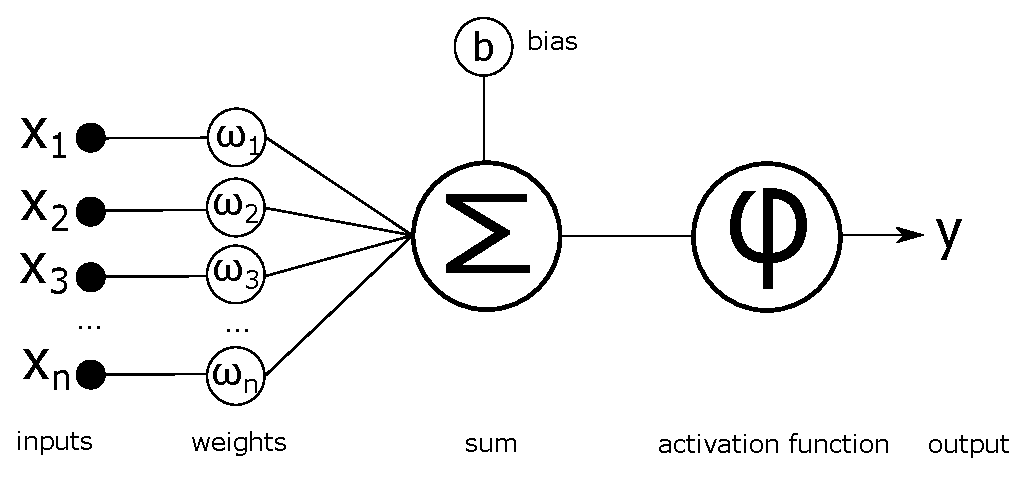
\includegraphics[width=10cm]{neuron.eps}
	\centering
	\caption{Symbolic structure of an artificial neuron.}
	\label{neuron_structure}
\end{figure}

\subsection{Layer}
\paragraph{}
Generally speaking, a layer represents an arbitrary transformation of input data inside the neural network. It is the essential building block of the neural network model in many deep learning frameworks (Tensorflow, Keras and et cetera). An organization of layers forms a computational graph defining operations performed on data. Layers do not even have to consist of any artificial neuron at all since a layer can be defined using other mathematical operation over the input data. However, the rest of this subsection is going to discuss a \textit{dense} layer, which is made up of the neurons introduced in section \ref{aritificial_neuron}.

\paragraph{}
When neurons are organized into the layer, it is not necessary to compute an output activation of each neuron one by one. Instead, the vector form of the equation for one neuron can be used to calculate the activation of the whole layer (equation \ref{layer_computation}). $W^T$ then denotes a transposed matrix of all the weights in the layer, $x$ is a vector of inputs and $b$ is a vector of biases \cite{Nielsen}. The function $\varphi$ is the activation function and is applied element-wise on the resulting vector $W^T x + b$. 

\begin{equation}
y = \varphi(W^T x + b)
\label{layer_computation}
\end{equation}  

Equation \ref{layer_computation_example} shows a detailed expansion of equation \ref{layer_computation} for a layer made up of two neurons and three inputs. In the expanded equation, $y_i$ denotes an output activation of the $i$-th neuron, $w_{ij}$ indicates a weight of the $j$-th input in the $i$-th neuron, $b_i$ is a bias of the $i$-th neuron and finally, $x_j$ represents a value of the $j$-th input \cite{Nielsen}. 

\begin{equation}
\begin{bmatrix}
y_1 \\
y_2
\end{bmatrix} =
\varphi(
\begin{bmatrix}
w_{11} & w_{12} & w_{13}\\
w_{21} & w_{22} & w_{23}
\end{bmatrix}
\begin{bmatrix}
x_1 \\
x_2 \\
x_3
\end{bmatrix} + 
\begin{bmatrix}
b_1 \\
b_2
\end{bmatrix}
)
\label{layer_computation_example}
\end{equation}  

\subsection{Model}
\paragraph{}
The way how different layers are organized and connected (figure \ref{nn_model}) is called a neural network model. Generally, a model consists of three parts - an input layer, hidden layers and an output layer. The input layer stands at the very beginning of the network and represents an entry point for data. If the input is an $N$-dimensional vector, then the input layer has $N$ neurons inside. Moreover, the first layer is simplified and does not perform any computation. The only thing done is that the output activation of each neuron is set to the value of the corresponding input ($y_i = x_i$). Subsequent layers (\textit{hidden layers}) perform the main part of the computation (section \ref{forwardpass}). Finally, activations in the output layer, which stands at the end of the model, are used to determine a resulting class (section \ref{forwardpass}). 

\begin{figure}[!h]
	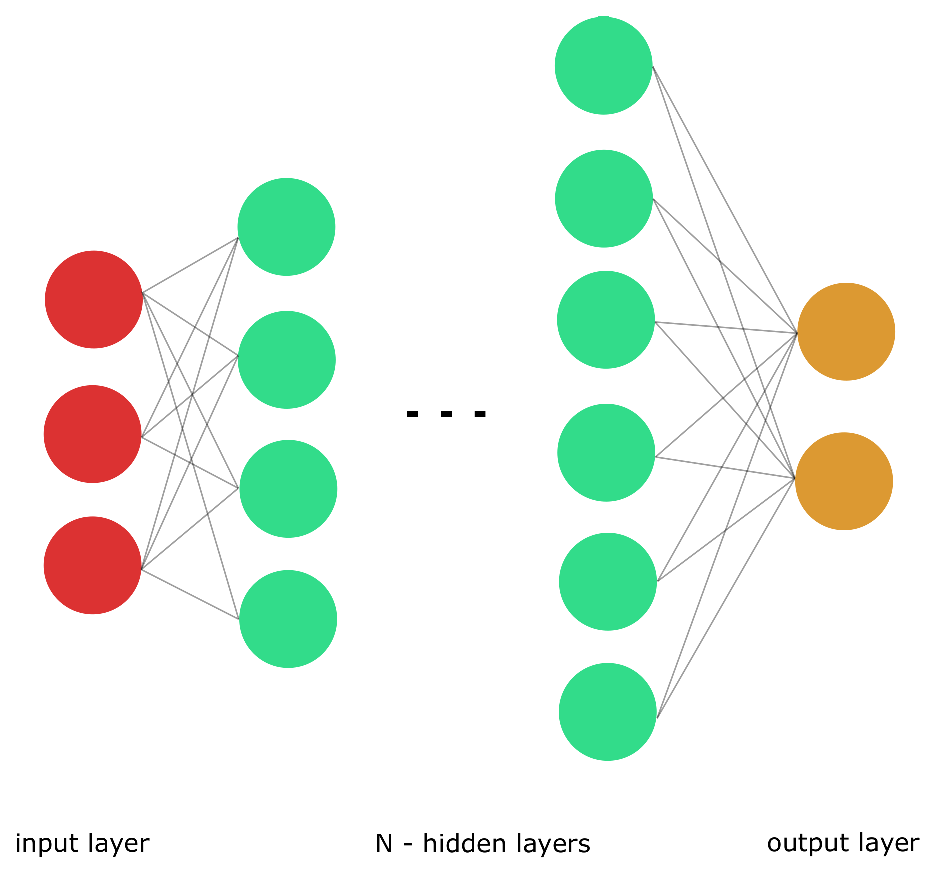
\includegraphics[width=10cm]{model.eps}
	\centering
	\caption{Example of a neural network model with four inputs, N hidden fully connected layers and two neurons at the output.}
	\label{nn_model}
\end{figure}

\section{Activation Functions}\label{activation_function}
\paragraph{}
An essential part of each neural network is a non-linear activation function, which is used to obtain the activation of a neuron/layer (equation \ref{neuron_computation}). Its most significant contribution is introducing a non-linearity into the model. Without such function, the neural network would be able to model only a linear dependency of a class on input data. It is because the output of the model would then consist of a linear combination of the input and the network parameters only \cite{deep_learning_with_python}.

\subsection{Sigmoid}
\paragraph{}
A sigmoid function (equation \ref{sigmoid_activation_eq}) is commonly used in output layers for tasks such as logistic regression or multi-label classification tasks. However, it is suitable for hidden layers as well \cite{python_ml_2nd}. Its major drawback is a vanishing gradient (draws near zero) for low and high values of the $z$. 

\begin{equation}
\varphi(z) = \frac{1}{1+e^{-z}}
\label{sigmoid_activation_eq}
\end{equation} 

\subsection{Hyperbolic Tangent (TanH)}
\paragraph{}
A hyperbolic tangent (equation \ref{tanh_activation_eq}) is similar to the sigmoid function in its shape and drawbacks, with the difference that a range of values is $<\!-1, 1\!>$, whereas sigmoid's range is $<\!0, 1\!>$. This activation function is predominantly used in hidden layers \cite{activation_functions_article}.

\begin{equation}
\varphi(z) = \frac{e^z - e^{-z}}{e^z + e^{-z}}
\label{tanh_activation_eq}
\end{equation} 

\subsection{Rectified Linear Unit (ReLU)}
\paragraph{}
A rectified linear unit is a straightforward activation function, which is defined as a maximum of zero and $z$. A significant advantage of ReLU is that it is computationally efficient and despite its simplicity, it turns out to work very well for a wide range of tasks. It is typically used in hidden layers \cite{python_ml_2nd}.

\begin{equation}
\varphi(z) = max(0, z)
\label{relu_activation_eq}
\end{equation} 

\subsection{Softmax}\label{softmax}
\paragraph{}
A softmax function (equation \ref{softmax_activation_eq})\cite{ml_probabilistic} is frequently used in output layers of the neural network thanks to its ability to transform the inputs into a probability distribution for the classes. It means that a sum of the softmax's output vector elements is always equal to one. In combination with a cross-entropy loss, it forces the network to give the highest predicted probability to the class given by the label and to assign as low probability as possible to the rest of them. 

\paragraph{}
It is worth mentioning that including the softmax in the activation functions section is questionable. It is due to the impossibility to compute an activation of a single neuron using the softmax. This fact can be seen in equation \ref{softmax_activation_eq}, where the knowledge of an inner product $z_j$ (bias added to the weighted sum) of all the neurons in the layer is necessary to scale the inner product of the current ($i$-th) neuron $z_i$. Therefore the softmax is often perceived as a self-standing softmax layer.

\begin{equation}
\varphi(z)_i = \frac{e^{z_i}}{\sum_{j=1}^{K} e^{z_j}}
\label{softmax_activation_eq}
\end{equation} 

\section{Classification Using a Neural Network}\label{forwardpass}
\paragraph{}
A classification task can be defined as a process of feeding in one sample of data, passing it through the whole model and determining the resulting class. This process is called a forwardpass and starts with setting output activations of neurons in the input layer according to values of the input. Then, the activation of the input layer is used as an input for the subsequent hidden layer. Generally, activation of the $n$-th layer is used as an input for the ($n+1$)-th layer. This step is done repeatedly until the output layer is reached.

\paragraph{}
Finally, when the activation of neurons in the output layer is known, a resulting class can be determined. Let us say that each neuron in the output layer represents one class, then a result of the classification is the one with the highest activation. 

\section{Loss/Cost Functions}\label{loss_function}
\paragraph{}
As further explained in section \ref{training}, the loss function is used during training as a measure of how good or bad the current setting of network parameters is. It should be noted that the value of the loss is not a suitable measure of a network accuracy. For this purpose, metrics introduced in section \ref{metrics} shall be used. Moreover, the selection of the loss function should be tailored to the metric we want to maximize, due to uncorrelation between some losses and metrics (section \ref{f1_loss}).

\subsection{Mean Squared Error}\label{MSE}
\paragraph{}
Mean squared error (MSE) is a loss function that is defined by equation \ref{MSE_eq} and suits well for regression tasks \cite{deep_learning_with_python}. In the equation, $C$ denotes the loss function, $w$ and $b$ are sets of all weights and biases of the neural network, respectively and $X$ is the current batch of inputs. On the right-hand side, there is a sum of the differences of labels $y$ and predicted values $\hat{y}$ summed over all inputs in the batch. Finally, the sum is divided by the number of examples $n$.

\begin{equation}
C(w, b, X) = \frac{1}{n}\sum_{x}^{} (y - \hat{y})^2
\label{MSE_eq}
\end{equation} 

\subsection{Cross-Entropy}\label{cross_entropy}
\paragraph{}
Another kind of a loss function is a cross-entropy loss (equation \ref{cross_entropy_eq}), which is often used for classification problems \cite{deep_learning_with_python}. The left side of the equation is identical to equation \ref{MSE_eq} and is described in section \ref{MSE}. On the right side, there is a negative-sum of product $y_{c}log(p_{c})$ over all possible classes $M$. In the product, $y_{c}$ is a binary class indicator - equal to 1 if the true class of a current sample is $c$, else 0. Finally $p_{c}$ is a probability of the current sample belonging to class $c$ \cite{cross_entropy}. Value of $p_{c}$ is determined by a softmax output layer (section \ref{softmax}) with which, the cross-entropy should be used.

\begin{equation}
C(w, b, X) = -\sum_{c=1}^{M} y_{c}log(p_{c})
\label{cross_entropy_eq}
\end{equation} 

\subsection{F1 Loss}\label{f1_loss}
\paragraph{}
In some cases, it might happen that the loss value does not correlate with a metric meant to be maximized. In other words, even if the loss decreases, the maximized metric may decrease as well. However, the expectation is that if we get better (lower) loss, we get a better (higher) value of the metric. This phenomenon can appear when the maximized metric is an f1 score (section \ref{f1_score}) and the chosen loss is a cross-entropy \cite{f1_loss}. In situations such as this, it is necessary to select another loss function, which can result in a better-trained model.

\paragraph{}
To maximize the f1 score (section \ref{f1_score}) it can be favorable to use the f1 loss. Equation \ref{f1_loss_eq} states how the f1 loss is calculated. The equation is the same as in the case of the f1 score. However, the meaning of $TP$ (true positives), $FP$ (false negatives), $FN$ (false negatives) is different from the f1 score. That is to be able to differentiate the loss. For example, if a label is $1$ and a model's prediction is $0.8$ probability for class $1$, we count $TP=0.8*1$, $FN=0.2*1$ and $FP=0.8*0$. Generally, this calculation is described by equations \ref{f1_loss_partials_eq} \cite{f1_loss_towards}.

\begin{equation}
C(w, b, X) = \frac{1}{n}\sum_{x}^{}(\frac{2TP}{2TP+FP+FN})
\label{f1_loss_eq}
\end{equation} 

\begin{equation}
\begin{gathered}
TP = prediction * label \\
FN = (1 - prediction)*label \\
FP = prediction * (1-label)
\label{f1_loss_partials_eq}
\end{gathered}
\end{equation} 

\section{Training a Neural Network Model}\label{training}
\paragraph{}
Thanks to equation \ref{layer_computation} and a description of the forwardpass in section \ref{forwardpass}, it shall be clear that a result of classification is a function of input values, weights and biases. Since the input values are fixed, the only way how to affect the behavior of a neural network model is to adjust the weights and biases. The weights and biases are called parameters of the network.

\paragraph{}
The process of setting the weights and biases (which may be randomly initialized at the begging) to maximize the accuracy of the network is called training. To measure how optimal our current setting is, we define a loss function (section \ref{loss_function}). A higher value of the loss means a worse accuracy of the network. In other words, we try to minimize the loss. However, the loss is a function of thousands of variables (mostly network parameters),
which is the reason why it is not possible to find optimal values for all the
parameters analytically. Due to that, an approximation of the loss minimum
has to be found using gradient optimization methods (see section \ref{optimizers} for details).

\paragraph{}
The training procedure (minimizing the loss) is described in the following steps, which are performed in a loop over all dataset batches \cite{deep_learning_with_python}:

\begin{enumerate}
	\item Select a batch of training examples from a training dataset.
	\item Do a forward pass with the selected examples and get predictions.
	\item Compute the value of a loss over the current batch using the obtained predictions and true labels.
	\item Compute an error of each neuron in an output layer using the loss.
	\item Propagate the error to previous layers (this process is called a backpropagation).
	\item Adjust parameter values to minimize the error (minimize the loss).
\end{enumerate}

The loop over all the batches is performed multiple times (\textit{epochs}). Since the previous steps are only a brief description of the training process, refer to the book by M. Nielsen \cite{Nielsen} for further details.

\subsection{Optimizer}\label{optimizers}
\paragraph{}
An optimizer represents an exact algorithm that is used for adjusting the network parameters \cite{deep_learning_with_python}. Generally, the optimization is based on computing a gradient (direction of the steepest increase) for each parameter with respect to the loss. The calculated gradient is used to move a value of the parameter against the gradient direction by a certain amount of the gradient's size. The amount of change is called a learning rate and is denoted as $\eta$. The learning rate is a member of a particular  group of parameters called hyperparameters. They represent network parameters that are not learned during the training.

\paragraph{}
Examples of commonly used optimizers are listed below:

\begin{itemize}
	\item Stochastic gradient descent (SGD) \cite{sgd}
	\item RMSProp \cite{RMSprop}
	\item AdaGrad \cite{adagrad_paper}
	\item Adam \cite{Adam_paper}
\end{itemize}

\section{Metrics}\label{metrics}
\paragraph{}
As stated in section \ref{loss_function}, a loss function is not the best for measuring how well a network is trained. For this purpose, it is necessary to use other metrics that are presented in this section.

\subsection{Accuracy}\label{accuracy}
\paragraph{}
Accuracy is defined as a fraction of correctly classified examples (equation \ref{accuracy_eq}). Even though this metric is the most often used one, it is not suitable for datasets with an unbalanced number of samples in the classes. For instance, if there is a binary classification task and we have a dataset with 95\% of "true" examples, the classifier can achieve a 95\% accuracy only by classifying all the data as "true". It means that it might be reasonable to use another metric, such as an f1 score (section \ref{f1_score}), that does not suffer from this drawback.

\begin{equation}
acc = \frac{\: correctly\: classified}{total\: number\: of\: examples}
\label{accuracy_eq}
\end{equation} 

\subsection{Precision, Recall and F1 score} \label{f1_score}
\paragraph{}
Before defining what a precision, recall and f1 score are, it is necessary to establish the concept of true positives (TP), true negatives (TN), false positives (FP) and false negatives (FN), which are possible results of a binary classification. Table \ref{result_classes_f1} states the individual cases and assigns a correct result class (TP, TN, FP, or FN) to them \cite{python_ml_2nd}. 

\begin{table}[h!]
	\centering
	\begin{tabular}{c c c} 
		\hline
		Label & Prediction & Result class \\ [0.5ex] 
		\hline\hline
		1 & 1 & TP \\ 
		1 & 0 & FN \\
		0 & 1 & FP \\
		0 & 0 & TN \\ [1ex] 
		\hline
	\end{tabular}
	\caption{Possible results of binary classification and underlying result classes.}
	\label{result_classes_f1}
\end{table}

\paragraph{}
Using the previously declared result classes, the precision, recall and the f1 score can be defined. The precision (equation \ref{precission_eq}) is a fraction of correctly classified positive samples from all samples classified as positive (equation \ref{recall_eq}). The recall is a fraction of correctly classified positive samples from all the truly positive samples. Finally, the f1 score is defined as  a harmonic mean of precision and recall (equation \ref{f1_score_eq}). As stated in section \ref{accuracy}, the f1 score is extremely useful for the evaluation on unbalanced datasets. 

\begin{equation}
precision = \frac{TP}{TP + FP}
\label{precission_eq}
\end{equation} 

\begin{equation}
recall = \frac{TP}{TP + FN}
\label{recall_eq}
\end{equation} 

\begin{equation}
f1\_score = 2\:\frac{precission*recall}{precission+recall}
\label{f1_score_eq}
\end{equation} 

\paragraph{}
Even though the stated computation works for binary classification only, there are three possible ways of how to generalize the f1 score for multi-class classification. This generalization can be made using a micro, macro and weighted f1 score \cite{multiclass_f1_score}.

\subsection{Confusion Matrix}
\paragraph{}
A confusion matrix (figure \ref{conf_matrix_example}) is a handy metric for evaluating network behavior in detail. Its significant benefit is that it shows which classes are being confused during the classification. It means that the confusion matrix is a $C \times C$ sized matrix where each member $n_{ij}$ of the matrix denotes the number of cases when a sample of the $i$-th class was classified as the class $j$. Thanks to that, we can identify classes that the model struggles to distinguish the most. The confusion matrix may also appear in a normalized form, where each row is normalized to one.

\begin{figure}[!h]
	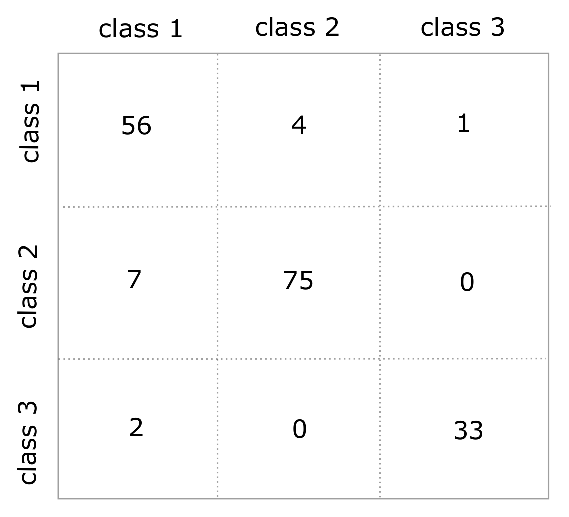
\includegraphics[width=7cm]{conf_matrix.eps}
	\centering
	\caption{An example of a confusion matrix for three-class classification. For example, it shows that a sample from class 2 was classified as a class 1 for seven times.}
	\label{conf_matrix_example}
\end{figure}

\section{Other Neural Network Concepts and Techniques}\label{other_nn_architectrues_and_techniques}
\paragraph{}
A concept of the multilayer perceptron does not suit very well for all tasks where neural networks can be utilized. Therefore, many other architectures dealing with different drawbacks of the original concept were developed. One such architecture, which tries to address a problem of multi layer perceptron's inability to deal with sequential data, is a recurrent neural network (RNN) \cite{RNN_LSTM} and its often used bi-directional form \cite{RNN_LSTM}. An extension of this concept is a gated recurrent unit (GRU) and a long short term memory (LSTM)\cite{colahs_lstm} network that can handle long term dependencies in the sequences. The concept of RNNs is often amended by an attention mechanism  \cite{colahs_attention}.

\paragraph{}
Another type of architecture is a convolutional neural network (CNN), which applies a convolution operation over a sliding window to discover patterns emerging in the input \cite{python_ml_2nd}. This concept is often used for image or video classification and natural language processing. 

\paragraph{}
Although these concepts are quite diverse, they all suffer from a common problem, which is overfitting \cite{Nielsen}. This phenomenon can be identified by achieving perfect training accuracy while having poor results on a validation part of the dataset. To cut down the influence of the overfitting, regularization techniques can be used. An example of a regularization technique is an L2 regularization \cite{Nielsen} or a dropout \cite{droupout_in_cnns}.

\subsection{Siamese Neural Networks}
\paragraph{}
The previously discussed multilayer perceptron can be perceived as a sequential network (figure \ref{sequential_neural_network}), since layers are organized into an ordered sequence that defines the flow of computation. However, the sequential network that accepts one input vector (or one sequence) is not the only type of neural network architecture. 

\begin{figure}[!h]
	\includegraphics[width=13cm]{sequential_nn.eps}
	\centering
	\caption{An example of a sequential neural network.}
	\label{sequential_neural_network}
\end{figure}

Generally, the neural networks can have multiple input vectors or sequences and the organization of the layers can be diverse. A special type of architecture is a siamese network \cite{siamese_nn}. This kind of network accepts two inputs that are passed through two parallel subnets sharing their weights. The two subnets can be followed by other layers processing an output of the subnets. An example of siamese network architecture is depicted in figure \ref{siamese_neural_network_fig}. Such architecture finds its usage, for example, in facial recognition or semantic similarity (section \ref{semantic_similarity_tasks}).

\begin{figure}[!h]
	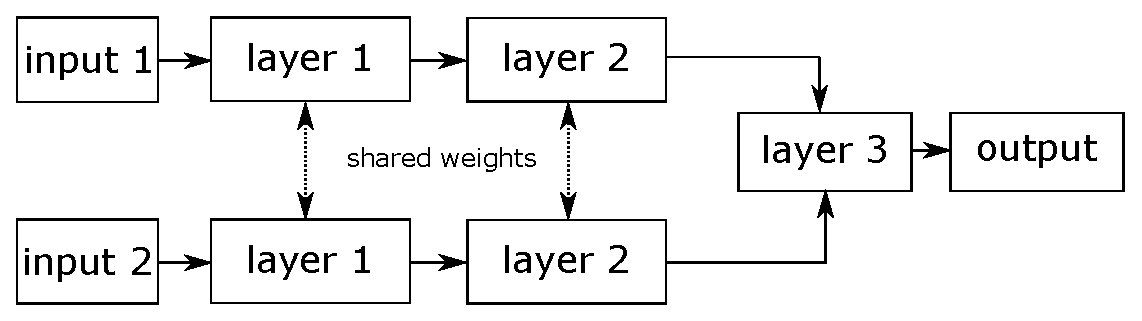
\includegraphics[width=13cm]{siamese_nn_overall.eps}
	\centering
	\caption{A siamese neural network that accepts two inputs and produces one output vector. The layers on the same level share their weights, as marked in the picture.}
	\label{siamese_neural_network_fig}
\end{figure}  

